\section{Introduction}

\begin{frame}
	\begin{block}{faiss}
		In this report, we cover results of our experiments with \texttt{faiss}\footnotemark \, library \cite{Johnson2017} for the nearest neighbors search. The report includes the following:
		\begin{itemize}
			\item Timing comparison for the k-means task on SIFT2M data evaluated before;
			\item k-NN graph construction with various indices from \texttt{faiss} and evaluation of timings and precision on Oxford105K data set.
			\item Implementation of the smooth path algorithm within the k-NN graph based on (12) of \cite{Johnson2017}. Oxford105K data was utilized.
		\end{itemize}
	\end{block}
	
	\begin{block}{Technical Details}
		The respective implementation is available on our \href{https://github.com/salisaresama/computer-vision}{{\color{blue}\underline{GitHub}}} page.
	\end{block}
	
	\addtocounter{footnote}{-1}
	\stepcounter{footnote}\footnotetext{We utilize Fair AI Similarity Search (\href{https://github.com/facebookresearch/faiss}{{\color{blue}\underline{faiss}}}) library with fixed parameters of the index: \texttt{nlist}$=256$, $m=16$, \texttt{nbits}$=8$, and \texttt{nprobe}$=32$ of IVFPQ index.}
\end{frame}


\section{$k$-means Task}
\subsection{Timing}


\begin{frame}

\begin{block}{Description}

Once again we perform naive $k$-means iterations on the SIFT2M data set with $k = 32000$. However, this time only exact nearest neighbors are searched for. Moreover, the search is done by means of GPU. As expected, the flat index from \texttt{faiss} on a GPU-enabled machine performs the search of nearest cluster centers more than a thousand times faster (recall that it took approx. 9K seconds before). Cluster assignment still takes relatively long, as it was not optimized for GPU by us.
	
\end{block}


	\begin{table}
		\small
		\begin{tabular}{| c || c | c |}
			\hline
			Title & (AVG. | STD.) NN time, [s] & (AVG. | STD.) assignment time, [s] \\
			\hline
			\hline			
			Exhaustive NN search& 2.58 | 0.37 & 136.56 | 18.36 \\
			\hline  
		\end{tabular}
	\end{table}
\end{frame}


\section{k-NN Graph}
\subsection{Timings}


\begin{frame}
	
\end{frame}


\subsection{Precision Evaluation}


\begin{frame}
	
\end{frame}


\subsection{Paths}


\begin{frame}
\begin{block}{Smooth Path Evaluation}
	Another exercise we have performed in the scope of this work is the implementation of the path search given by equation (12) in \cite{Johnson2017}. We have utilized a depth-first search with cut-off to generate simple paths in the k-NN graph. To stress the preference on path smoothness, the choice was made according to cost function $\min_{P} max_{i} d_{p_{i}, p_{i+1}}$ where $P = (p_{1}, p_{2}, \dots, p_{n})$ denotes paths between the source and the target and $n <$ cut-off value. An example is shown in Fig.~\ref{fig:smooth_path}.
\end{block}

\end{frame}


\begin{frame}

\begin{figure}
\centering
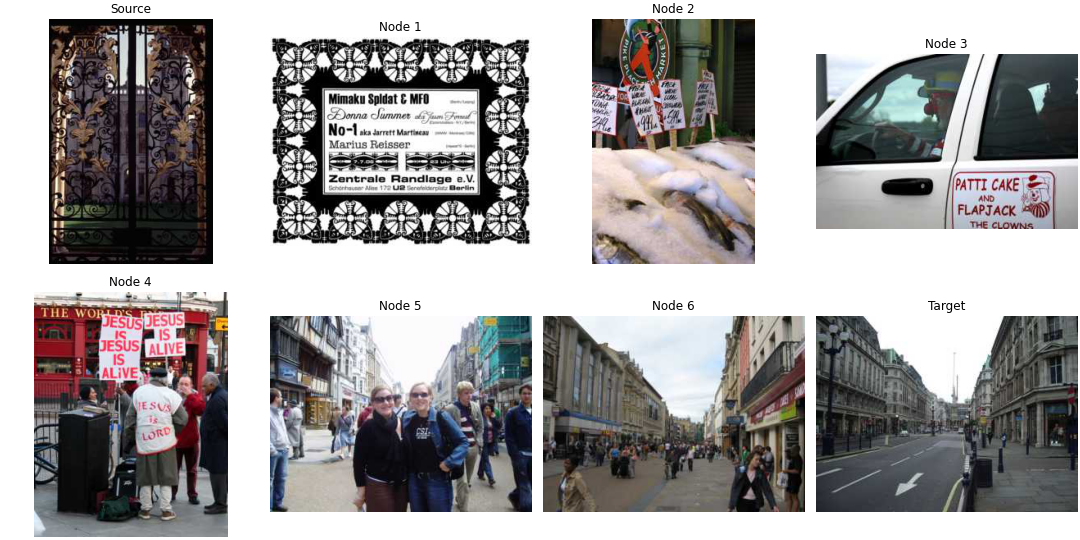
\includegraphics[width=0.85\linewidth,height=0.65\textheight]{../images/knn/path}
\caption{Sample of the smooth path search between the source image and the target image within the exact 10-NN graph of the whole Oxford105K data set; cut-off value was set to 7.}
\label{fig:smooth_path}
\end{figure}

\end{frame}